\documentclass[11pt,a4paper]{article}
\usepackage[text={6.5in,10in},centering,a4paper]{geometry}
\usepackage{amssymb,amsmath} % Equations
\usepackage{tabularx} % Tables
\usepackage{graphicx,color} % Graphics, Figures
\usepackage[tight,footnotesize]{subfigure}
\usepackage{pgfgantt} % for gantt chart
\usepackage{indentfirst}
\usepackage{hyperref}
\usepackage{amsmath} % for large blaces
\usepackage{esvect} % easy vector

\graphicspath{{figures/}} % create a director 'figures' in your local dir and all pics are kept here

\title{
  \textbf{Senior Project Proposal 2102490 Year 2017}  \\[2ex]
  Analysis and Design of Planar Phased Array Antenna for \\[1ex]
  5 GHz Applications
}
\author{\textbf{Norawit Nangsue ID 5730289021} \\[1ex]
\textbf{Advisor: Assist. Prof. Tuptim Angkaew} \\[1ex]
\textbf{Department of Electrical Engineering, Faculty of Engineering} \\[1ex]
\textbf{Chulalongkorn University}
}
\date{\today}

\renewcommand\familydefault{\sfdefault} % set to San Serif series




\begin{document}
  \maketitle
  \tableofcontents
  \newpage
  \section{Introduction}
    \indent Nowadays, antennas have been using in every wireless communication systems. It have been found out that microstrip patch is one of the most popular\cite{AkS} in the world. Also, the patch antenna is cost-effective and easy to fabricate\cite{AtT}. Many design approaches have been revealed for antenna engineers to follow the procedure. In order to obtain the precise dimension, a deep analysis might've be engaged.
    \indent A phased array is the set of antennas that could be a formation as a line or a planar which could steer its beam electrically\cite{CoB:05} which means that the direction of the antenna can be control wthout moving any of the mechanic part. Therefore, this proposal is aiming on two of very interesting technologies in this era.

  \section{Objectives}
    \indent The propose of this work is mainly focus on analyzing and designing the 5.6 GHz planar phased array antenna based on methods which have been analyzed, formulated or derived in the past. 

  \section{Methodology}
    \indent This section will provide a full analysis of designing a microstrip antenna and a phased array antenna.

    \subsection{Dimension Design of the Microstrip Antenna}
      \indent a dimension of microstrip antenna can be designed easily with this expressions\cite{NoK:05}.
      \begin{equation}
        L = \frac{c}{2f_0\sqrt{\epsilon_r\mu_r}} - 2\Delta l 
        W = \frac{c}{2f_0}
      \end{equation}
      \indent where $L$ and $W$ are the dimensions of an antenna\\[1ex]
      \indent $f_0$ is the resonance frequency\\[1ex]
      \indent $\epsilon_r$ is the relative dielectric constant\\[1ex]
      \indent $\mu_r$ is the relative magnetic constant\\[1ex]
      \indent $c$ is the speed of light in free space\\[1ex]
      \indent $\Delta l$ is the fringing effect at the edge of the antenna
      \indent However from \cite{CoB:05} the best width should be
      \begin{equation}
        W = \frac {1} {2 f_r \sqrt{\mu_{0} \epsilon_{0}}}\sqrt{\frac{2}{\epsilon_{r} + 1}} = \frac{\upsilon_{0}}{2f_{r}}\sqrt{\frac{2}{\epsilon_{r} + 1}}
      \end{equation}
      \indent where $\upsilon_{0}$ is the free-space velocity of light

    \subsection{Fringing Effect of the Microstrip Antenna}
      \subsubsection {Length Extension} 
      \begin{equation}
        \frac{\Delta l}{h}=0.412\frac{(\epsilon_{r(eff)}+0.3)(\frac{W}{h} + 0.264)}{(\epsilon_{r(eff)}-0.258)(\frac{W}{h} + 0.8)}
      \end{equation}
      \indent The length is extended by $\Delta L$ on both side so $L_{eff} = L + 2\Delta L$

    \subsection{Resonance frequency}
      \indent In $TM_{010}$ mode, the resonant frequency is given by
      \begin{equation}  
        f_{r(010)} =  \frac{1}{2 L\sqrt{\epsilon_{r}}\sqrt{\epsilon_{\mu_{0}\epsilon_{0}}}}= \frac{\upsilon_{0}}{2L\sqrt{\epsilon_{r}}}
      \end{equation}
      \indent With fringing effect, the equation will be given by
      \begin{equation} 
        f_{r(010)} =  \frac{1}{2 L_{eff}\sqrt{\epsilon_{r(eff))}}\sqrt{\epsilon_{\mu_{0}\epsilon_{0}}}}=\frac{1}{2(L + 2\Delta L)\sqrt{\epsilon_{r(eff)}}\sqrt{\epsilon_{\mu_{0}\epsilon_{0}}}}
      \end{equation}

    \subsection{Q Factor}
    \indent There are 4 main loss that should be considered\cite{NoK:05}
      \begin{itemize}
        \item $Q_{rad}$ is radiation loss due to a loss which propagates into a space
          \begin{equation}
            %\begin{aligned}
              Q_{rad} = \frac{3}{16}\frac{\epsilon_r}{p}\frac{a_e}{b_e}\frac{\lambda_0}{h}\frac{1}{1-\frac{1}{\epsilon_r\mu_r}+\frac{2}{5\epsilon_r^2\mu_{r}^2}}
            %\end{aligned}
          \end{equation}
          \indent where $a_e$,$b_e$,$h$ is the effective length, width and thickness of the antenna respectively,
           $p$ is the ratio of the power that radiated by the patch antenna to the power radiated by an equivalent dipole\cite{NoK:05}
        \item $Q_{sw}$ is surface-wave loss which represents the amount of power coupled into space waves
          \begin{equation}
            Q_{sw} = Q_{rad}(\frac{\eta_r^0}{1-\eta_r^0})
          \end{equation}
          \indent where $\eta_r^0$ is the radiation efficiency without dielectric or conductor loss
        \item $Q_d$ is dielectric loss which defined as the ratio (or angle in a complex plane) of the lossy reaction to the electric field E in the curl equation to the lossless reaction
          \begin{equation}
            Q_d = \frac{1}{\tan\delta}
          \end{equation}
        \item $Q_c$ is metalization loss
        \begin{equation}
          Q_c = h\sqrt{\mu\pi{f}\sigma}
        \end{equation}
      \end{itemize}
    \indent The total quality factor of the antenna can be given by using this formula.
      \begin{equation}
        \frac{1}{Q} = \frac{1}{Q_{rad}} + \frac{1}{Q_{sw}} + \frac{1}{Q_d} + \frac{1}{Q_c}
      \end{equation}

    \subsection{Radiation Resistance}
      \indent Radiation Resistance defines how 
        \begin{equation}
          %%\frac{1}{Q} \cong \frac{1}{Q_{rad}} + \frac{1}{Q_{sw}} + \frac{1}{Q_d} + \frac{1}{Q_c}
        \end{equation}
    \subsection{Bandwidth}

    \subsection{Radiation Pattern}
    
  \newpage

    \subsection{Transmission Line Model}
      \indent Transmission Line Model is considered as the easiest way to analyze the description of the
              rectangular microstrip patch.
      \begin{figure}[ht]
        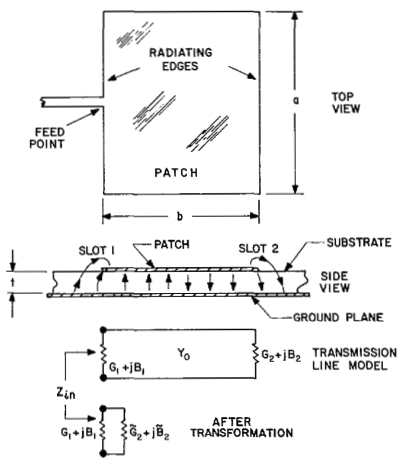
\includegraphics{tmmodel.png}
          \centering
          \caption{The antenna at top view, side view, and its transmission line model\cite{CaM:81}}
          %\label{fig:10}
      \end{figure}

      \subsubsection{Slot admittance}
        \indent The slot admittance is given by \cite{CaM:81}
        \begin{equation}
          G_1 + jB_1 \cong \frac{\pi {a}}{\lambda_0 z_0}[1 + j(1-0.636\ln{k_0w})]
        \end{equation}
        \indent where $a$ is the length of the patch antenna, $\lambda_0$ is free space wavelength,
                $k_0 = frac{2\pi}{\lambda_0}$, and $w$ is the slot width which is approximately
                equals to the thickness of the substrate $t$ 

      \subsubsection{Characteristic admittance}
        \indent Assume that there is no field variation along the edge of plate, so the characteristic admittance is given by \cite{CaM:81}
        \begin{equation}
          Y_0 = \frac{a\sqrt{\epsilon_r}}{tz_0}
        \end{equation}
        \indent where $t$ is the substrate thickness and the impedance of free space which is $\sqrt{\frac{\mu_0}{\epsilon_0}}$

      \subsubsection{Total Admittance \& Resistance at Resonance frequency}
        \indent By using Smith chart to get the length that will reflute out the imaginary part. Then, the total impedance would be
        \begin{equation}
          Y_{in} = 2G_1
        \end{equation}
        \indent Typically, $b$ should be at $0.48\lambda_d$ to $0.49\lambda_d$ because of the imaginary part reflution
                and the compensation of the fringing effect that cause an extra effective length. Also, $a$ should be around
                $0.5\lambda_0$ as well to get the best power radiation.  \\[1ex]
        \indent After complete the calculation of the admittance from the above parameters, so that the admittance
                $G_1 = 0.00417$ mhos. Then the input impedance of the antenna would be
        \begin{equation}
          Z_{in} = \frac{1}{2G_1} = 120 \indent \Omega
        \end{equation}

      \subsubsection{Resonance frequency}
        \indent The resonant frequency is found from
        \begin{equation}
          f_r = \frac{c}{\lambda_d\sqrt{\epsilon_r}} = q\frac{c}{2b\sqrt{\epsilon_r}}
        \end{equation}
        \indent where $q$ is the accurary of the resonant frequency and could easily determined by measuring $f_r$ \cite{CaM:81}
      
        \subsubsection{Summary}
        \indent The transmission line model is very easy to design and calculate parameters. However, the transmission line
                model is hardly to adapt with the other shape of the patch or. Also, this model is lack of accurate data.
                In order to find more precise infomation about the antenna, the Cavity model will be introduced 
                in the next section which is much more accurate than this one.\cite{CaM:81,NoK:05}
  \newpage

    \subsection{Cavity Line Model}
    \indent The cavity model has more accurate formulation for the input impedance, resonance with a little
            increase of mathematical complexity.\cite{CaM:81}
    \begin{figure}[ht]
      \label{cavitymodel}
      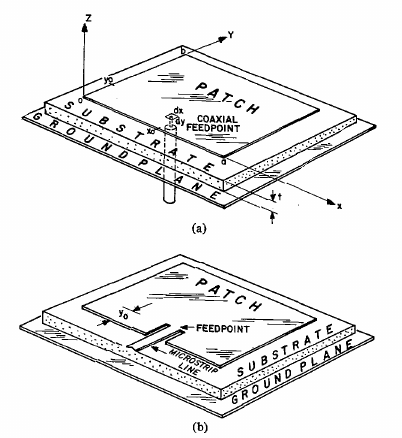
\includegraphics{cavitymodel.png}
      \centering
      \caption{(a) Microstrip patch with inset coaxial feed
               (b) Microstrip patch with inset transmission-line feed
              }
    \end{figure}

      \subsubsection{General form of electric field}
        \indent Considering a rectangular patch with width $a$ and length $b$ over a ground plane with $t$ substrate
                thickness and a dielectric constant $\epsilon_r$. With the relatively short thickness of the substrate,
                the electric field will be in z-direction with $TM_{mn}$ interior modes so that\cite{CaM:81}
        \begin{equation}
          E_z = \sum_m\sum_n A_{mn}e_{mn}(x,y)
        \end{equation}
        \indent where $A_{mn}$ are the mode amplitude coefficients and $e_{mn}$ are z direction electric mode vectors.
        \indent However, the mode that is used in the antenna is just only $TM_{10}$ so the equation can easily write as
        \begin{equation}
           E_z = A_{10}e_{10}(x,y)
        \end{equation}

      \subsubsection{Nonradiating cavity with perfect open-circuit wall equation of electric field}
        \indent With a calculation from boundary condition, it could be found that
          \begin{equation}
            e_{mn}(x,y) = \frac{\chi_{mn}}{\sqrt{\epsilon abt}}\cos{k_nx}\cos{k_my}
          \end{equation}
        \indent with
          \begin{equation}
            \chi_{mn}=
            \begin{cases}
              1       , & m = 0\quad     \text{and}\quad  n = 0 \\
              \sqrt{2}, & m = 0\quad     \text{ or }\quad  n = 0 \\
              2       , & m \neq 0\quad  \text{and}\quad  n \neq 0
            \end{cases}
          \end{equation}

      \subsubsection{Wavenumber}
        \indent The homogenous wave function and the eigenvalues must be complied with the seperation equation
        \begin{equation}
          k_{mn}^2 = \omega_{mn}^2\mu\epsilon = k_n^2 + k_m^2\\
        \end{equation}
        \indent in the case of nonradiating cavity
        \begin{equation}
          k_{n} = \frac{n\pi}{a}\\
          k_{m} = \frac{m\pi}{b}
        \end{equation}

      \subsubsection{Nonradiating cavity with perfect open-circuit wall equation of magnetic field}
        \indent From Maxwell-Faraday equation
        \begin{equation}
          \nabla \times \vv{E} = - \frac {\partial{\vv B}} {\partial t}
        \end{equation}
        \indent or in phasor form,
        \begin{equation}
          \nabla \times \vv{E} = -j\omega{\vv B}
        \end{equation}
        \indent after substitute the electric field equation, the magnetic field will be
        \begin{equation}
           \vv{h}_{mn} = \frac{1}{j\omega\mu}\frac{\chi_{mn}}{\sqrt{\epsilon abt}}(\vv{x}k_m\cos{k_nx}\sin{k_my} - \vv{y}k_n\sin{k_n}{x}\cos{k_m}{y})
        \end{equation}
        \indent For nonradiating case, the boundary condition $\vv{n} \times \vv{h}_{mn} = 0$ is satisfied on every walls.
                But, in radiating case, $\vv{h}_{mn}$ will not have a zero tangential on the cavity sidewall anymore.
                However, those pertubation from radiating effect cause just a little error on $e_{mn}$\cite{CaM:81}
      
      \subsubsection{Mode Coefficient}
        \indent From z-direction current, with the current probe $I_{0}$ at the location $(x_0,y_0)$ as in the
                figures illustrates in \ref{cavitymodel}. The coefficients from each mode can be obtained from
        \begin{equation}
          A_{mn} = \frac{j\sqrt{\mu\epsilon}k}{k^2-k_{mn}^2} \int\int\int\vv{J} \cdot \vv{e}_{mn} dv
        \end{equation}
        \begin{equation}
          A_{mn} = jI_0 \sqrt{\frac{\mu t}{ab}} \frac{k\chi_{mn}}{k^2-k_{mn}^2} G_{mn} \cos{k_my_0}\cos{k_nx_0}
        \end{equation}

        \begin{equation}
          rrr
        \end{equation}



    \subsection{Phased Array Antena}
      In phased array antenna principle, there are 2 main factor in the equations. First one is an element factor which is the factor that come from only one antenna itself and the another factor is called array factor which is come from the effect of multiple antennas combining together.
      \begin{equation} 
        S(\vartheta)=S_{e}(\vartheta)S_a(\vartheta)  \label{ii}
      \end{equation}
        Whereas \\[1ex]
        \indent $S_{e}$ is a radiation pattern from only one element\\
        \indent $S_{a}$ is a element factor with
        \begin{equation} 
          S_{a}(\vartheta) = \sum\limits_{i=1}^K a_{i}e^{jk(K-i)dsin(\vartheta)}
        \end{equation}
        \indent $a_{i}$ is an amplitude taper.\\
        \indent $K$ is a number of array antenna.\\
        \indent $d$ is a distance of each antenna.\\
        \indent $\vartheta$ is a wavefront angle

  \pagebreak

  \section{Preliminary results}
    \indent This project results will consist of
    1) a simulation program that have ability  to simulate a microstrip from the given parameters.
    2) an phased antenna that could steer its direction to the desired point 
    
    \subsection{Simulation Application}
    \indent By using all the parameters that required to design the antenna, this simulation application will provide
    all the data from the algorithm that was proposed from the past. There are many techniques to simulate the antenna
    as Method of Moments(MoM) or Numerical Method. In order to inspect on its correctness, the standard simulation might
    be required. Consequently, the antenna results is expected to have similar outcomes as well.

    
    
    \subsection{Microstrip Antenna}
      \indent The result from a patch antenna should be have 
      \begin{figure}[ht]
        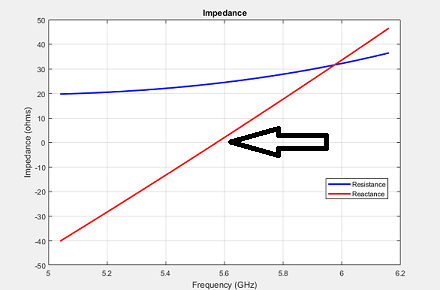
\includegraphics{Impedance.png}
        \centering
        \caption{The designed antenna's impedance should have approximately 0 Ohm reactance at 5.6 GHz}
        %\label{fig:1}
      \end{figure}

      \begin{figure}[ht]
        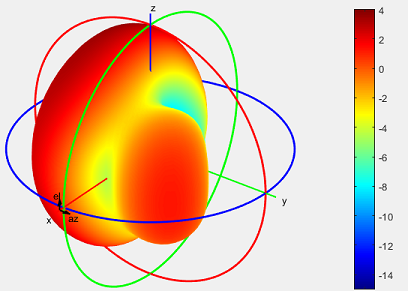
\includegraphics{Radiation_pattern}
        \centering
        \caption{The designed antenna's radiation pattern should have clear directivity}
        %\label{fig:2}
      \end{figure}

  \pagebreak

    \subsection{Array Antenna Patern}
      \begin{figure}[ht]
        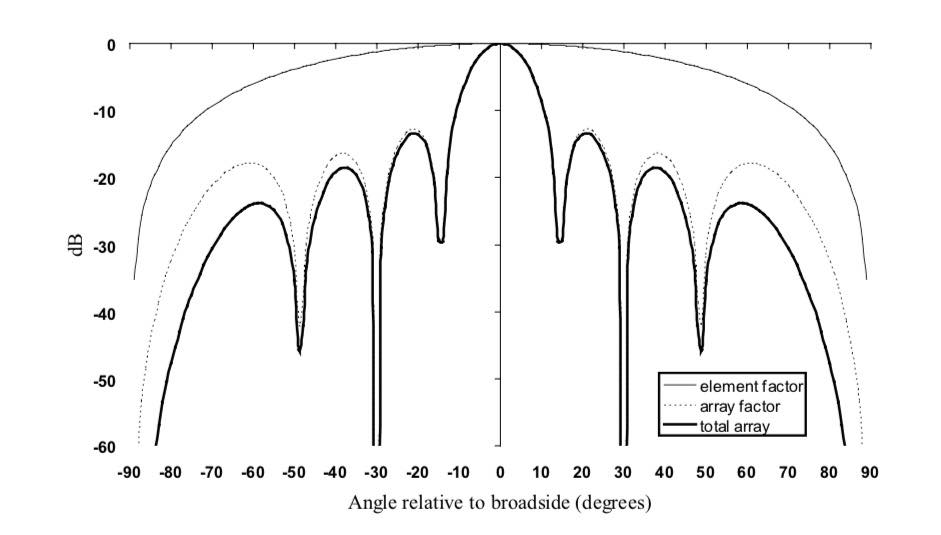
\includegraphics[scale=0.5]{no_taper}
        \centering
        \caption{Power radiation pattern without amplitude taper aka. $\forall a_{i} = 1$}
        %\label{fig:3}
      \end{figure}

      \begin{figure}[ht]
        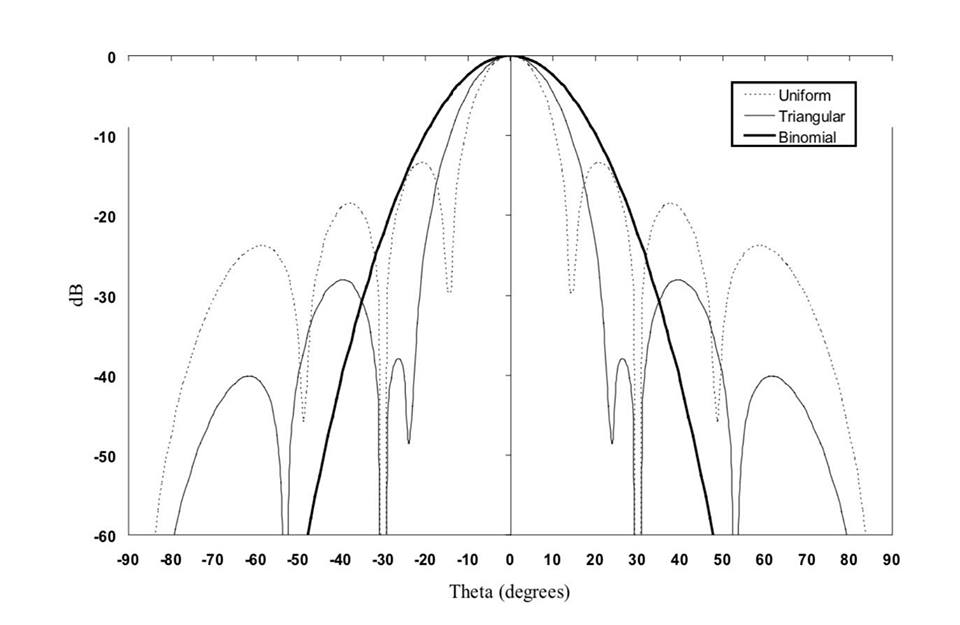
\includegraphics[ scale=0.5]{with_taper}
        \centering
        \caption{Power radiation pattern with amplitude taper of each type}
        %\label{fig:4}
      \end{figure}

  \pagebreak

  \section{Project overview}
    \subsection{Scope of work}
      \begin{itemize}
        \item An analysis of a microstrip antenna and phased array antenna
        \item A basic simulation application for finding antennas' radiation pattern
        \item A physical antenna device with its test result.
      \end{itemize}

    \subsection{Expected outcomes}
      \indent It's expected that the simulation application and the application that come from other author
      will have similar results. Also, the physical device will have a preliminary result like those simulation
      applications as well.
  
    \newpage

    \bibliography{ref} 
    \bibliographystyle{ieeetran}

\end{document}
